---
id: tkz-euclide-ejemplo-24
title: "Triángulo Isósceles Recto"
description: "Construye un triángulo isósceles rectángulo sobre una base y marca el ángulo recto."
keywords: [triangulo, isosceles, recto, angulo]
tags: [tkzDefTriangle, tkzDrawPolygons,tkzMarkRightAngles,tkzGetPoint]
sort: 24
---
\documentclass[tikz,border=2mm]{standalone}
\usepackage{tkz-base}
\usepackage{tkz-euclide}

\begin{document}
    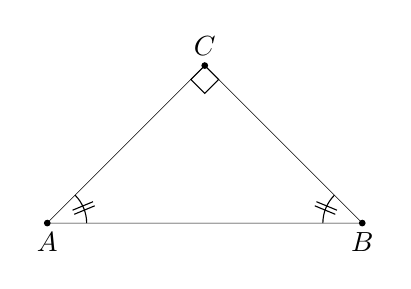
\begin{tikzpicture}
        % Define la base AB.
        \tkzDefPoint(0,0){A}
        \tkzDefPoint(4,0){B}
    
        % Construye un triángulo isósceles rectángulo en C usando AB como base.
        \tkzDefTriangle[isosceles right](A,B)
            \tkzGetPoint{C}
    
        % Dibuja el triángulo.
        \tkzDrawPolygons(A,B,C)
    
        % Marca el ángulo recto en C.
        \tkzMarkRightAngles(A,C,B)

        % Marca los ángulos en A y en B como congruentes
        \tkzMarkAngle[mark=||,size=0.5](B,A,C)
        \tkzMarkAngle[mark=||,size=0.5](C,B,A)
    
        % Dibuja y etiqueta los puntos.
        \tkzDrawPoints(A,B,C)
        \tkzLabelPoints(A,B)
        \tkzLabelPoints[above](C)
    \end{tikzpicture}
\end{document}
